\subsection{Model Animation}
\label{sec:MA}

To answer Challenge C2, it is important to design the MA framework with
the idea of reuse at its core. One possible approach is to separate two
things: the basic blocks defining animations \emph{effects} that may be combined
in comprehensive Model Animation Units (UAs), from the way they are organised
and scheduled to build complex animations. The approach we propose is similar
to the de-/reconstruction of MTLs described by \citet{J:SyrianiVangheluwe:2013}:
the idea is to capture the most basic animation effects, and offer powerful 
mechanisms to combine them, resulting in the ability to effectively specify any
kind of animation. We quickly discuss interesting effects before describing two
approaches for scheduling.

\begin{figure}[t]%
   \centering
   %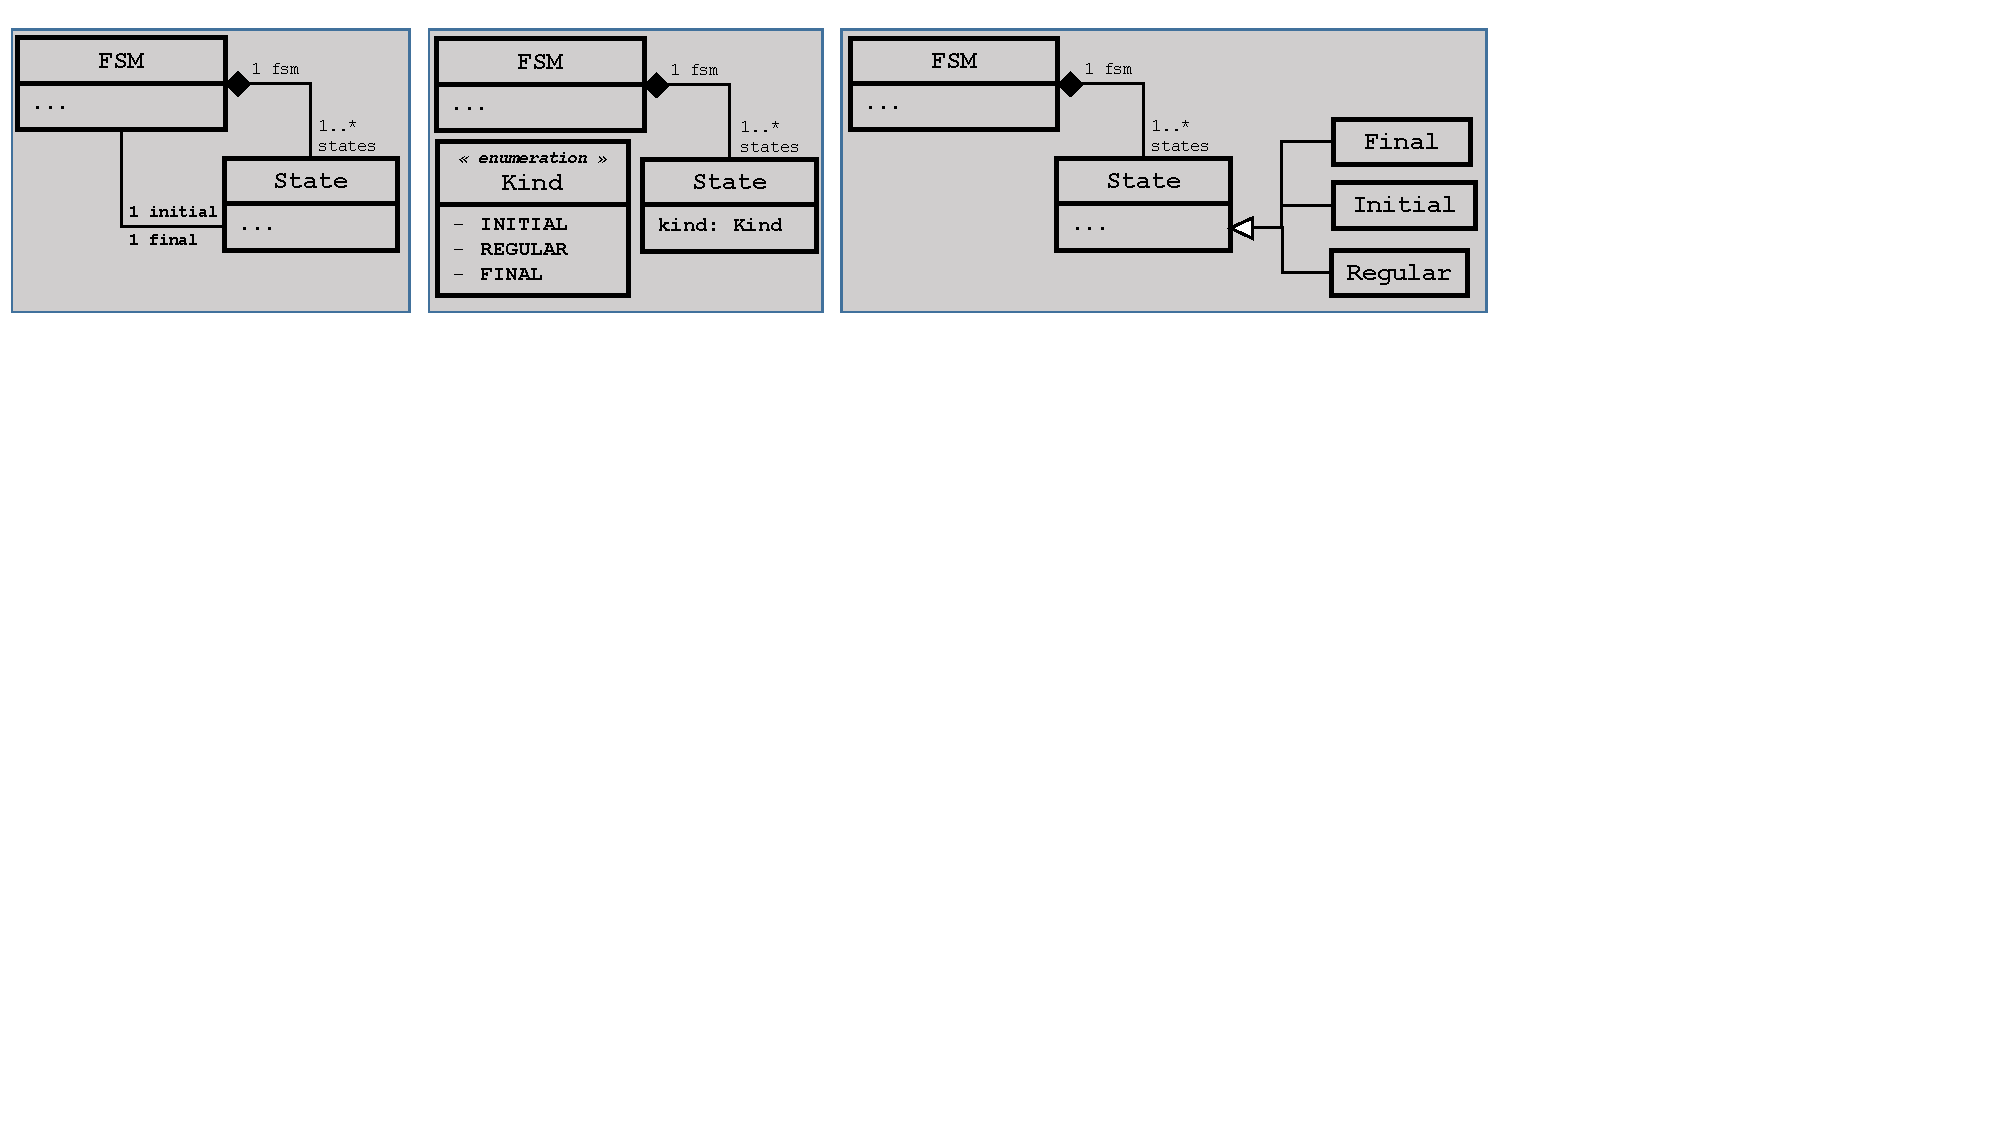
\includegraphics[width=\columnwidth,clip, trim=0cm 13.8cm 8.3cm 0.2cm]{FSM-Initial}%
   \caption{Two ways for UA scheduling: using embedding (left), and combinators (right).
   }%
   \label{fig:UA-Schedule}%
\end{figure}

\subsubsection{UA Effects}
\label{sec:MA-Effects}


\subsubsection{UA Scheduling}
\label{sec:MA-Scheduling}

Although theoretically equivalent, two approaches are possible for realising
this requirement.
\begin{description}
   \item[Embedding the scheduling \emph{inside} the UAs] As suggested in 
   \autoref{fig:UA-Schedule} (left), each UA is extended with pre- and 
   post-conditions. A precondition indicates how an UA starts relatively to the 
   previous one (at the same time, after, or delayed by a given time); while a
   postcondition would define whether the UA is repeated (and how many times).
   
   \item[Define \emph{combinators outside} of UAs] Another approach, suggested
   in \autoref{fig:UA-Schedule} (right) is to provide explicit \emph{combination}
   operators (aka. \emph{combinators}) that would take as operands UAs. Combinators
   similar to the previous case may be defined: sequencers with a possible delay,
   repetitors, and parallelisation. 
\end{description}
The second approach may seem more familiar to MA designers with a programming 
background, because the combinators approach proposes constructions similar to
what is available in GPLs. However, the first approach may be more compact visually,
and familiar for MA designers accustomed to slideshow tools such as Google Slides,
Microsoft Powerpoint or Apple Keynote.

Note that both approach may concurrently exist, allowing MA designers to choose
the most appropriate approach for specifying their MA. It is left as future work
to study under which conditions they may coexist (if possible at all), and to 
identify when and how each presents more benefits than the other.

